\documentclass[a4paper]{article}
\usepackage[utf8]{inputenc}
\usepackage{graphicx}
\usepackage{listings}
\usepackage{color}

\title{Approximating the exponential function}
\author{René Munk Thalund}
\date{March 2022}

\begin{document}
\maketitle
\begin{abstract}
We examine a \texttt{C\#} implementation of the exponential function that uses only multiplications and additions.
\end{abstract}

\section{Introduction}
The exponential function $e^x$ is ubiquitous in math and science. It's defined as the unique function that is it's own derivative, and has value 1 for argument 0, that is:

\begin{equation}
    \frac{df}{dx} = f(x) \; \textrm{and} \;  f(0) = 1
\end{equation}
The definition extends to complex arguments. Notably with an entirely imaginary argument $e^{i\phi} Z$ rotates the complex number Z by $\phi$ radians in the complex plane.


\section{Approximation}
We're considering the following \texttt{C\#}-function.

\begin{lstlisting}{language=[Sharp]C}
static double ex(double x){
    if(x<0)return 1/ex(-x);
    if(x>1.0/8)return Pow(ex(x/2),2);
    return 1+x*(1+x/2*(1+x/3*(1+x/4*(1+x/5*(1+x/
    6*(1+x/7*(1+x/8*(1+x/9*(1+x/10)))))))));
}
\label{code}
\end{lstlisting}
For small arguments $e^x$ is approximated using the geometric series up to the ninth term:

\begin{equation}
    \label{eq:regime1}
    e^x \approx \sum_{n = 0}^9 \frac{x^n}{n!} \; ,\;\;\; x \in [0,0.125]
\end{equation}
In the source code the sum us convoluted so the minimum number of multiplications and additions is used. For larger arguments $e^x$ is evaluated recursively, using the algebraic identity:

\begin{equation}
    \label{eq:regime2}
    e^x = (e^{x/2})^2, \;\; \textrm{used for}\;\;  x > 0.125
\end{equation}
As seen the argument is halfed in each recursion step until the regime defined by eq. \ref{eq:regime1} is reached. For negative arguments $e^x$ is evaluated as the reciprocal of the correponding positive argument:

\begin{equation}
    \label{eq:regime3}
    e^{-x} = \frac{1}{e^x} \;\; \textrm{used for}\;\;  x < 0
\end{equation}


\begin{figure}
    % GNUPLOT: LaTeX picture with Postscript
\begingroup
  \makeatletter
  \providecommand\color[2][]{%
    \GenericError{(gnuplot) \space\space\space\@spaces}{%
      Package color not loaded in conjunction with
      terminal option `colourtext'%
    }{See the gnuplot documentation for explanation.%
    }{Either use 'blacktext' in gnuplot or load the package
      color.sty in LaTeX.}%
    \renewcommand\color[2][]{}%
  }%
  \providecommand\includegraphics[2][]{%
    \GenericError{(gnuplot) \space\space\space\@spaces}{%
      Package graphicx or graphics not loaded%
    }{See the gnuplot documentation for explanation.%
    }{The gnuplot epslatex terminal needs graphicx.sty or graphics.sty.}%
    \renewcommand\includegraphics[2][]{}%
  }%
  \providecommand\rotatebox[2]{#2}%
  \@ifundefined{ifGPcolor}{%
    \newif\ifGPcolor
    \GPcolortrue
  }{}%
  \@ifundefined{ifGPblacktext}{%
    \newif\ifGPblacktext
    \GPblacktextfalse
  }{}%
  % define a \g@addto@macro without @ in the name:
  \let\gplgaddtomacro\g@addto@macro
  % define empty templates for all commands taking text:
  \gdef\gplbacktext{}%
  \gdef\gplfronttext{}%
  \makeatother
  \ifGPblacktext
    % no textcolor at all
    \def\colorrgb#1{}%
    \def\colorgray#1{}%
  \else
    % gray or color?
    \ifGPcolor
      \def\colorrgb#1{\color[rgb]{#1}}%
      \def\colorgray#1{\color[gray]{#1}}%
      \expandafter\def\csname LTw\endcsname{\color{white}}%
      \expandafter\def\csname LTb\endcsname{\color{black}}%
      \expandafter\def\csname LTa\endcsname{\color{black}}%
      \expandafter\def\csname LT0\endcsname{\color[rgb]{1,0,0}}%
      \expandafter\def\csname LT1\endcsname{\color[rgb]{0,1,0}}%
      \expandafter\def\csname LT2\endcsname{\color[rgb]{0,0,1}}%
      \expandafter\def\csname LT3\endcsname{\color[rgb]{1,0,1}}%
      \expandafter\def\csname LT4\endcsname{\color[rgb]{0,1,1}}%
      \expandafter\def\csname LT5\endcsname{\color[rgb]{1,1,0}}%
      \expandafter\def\csname LT6\endcsname{\color[rgb]{0,0,0}}%
      \expandafter\def\csname LT7\endcsname{\color[rgb]{1,0.3,0}}%
      \expandafter\def\csname LT8\endcsname{\color[rgb]{0.5,0.5,0.5}}%
    \else
      % gray
      \def\colorrgb#1{\color{black}}%
      \def\colorgray#1{\color[gray]{#1}}%
      \expandafter\def\csname LTw\endcsname{\color{white}}%
      \expandafter\def\csname LTb\endcsname{\color{black}}%
      \expandafter\def\csname LTa\endcsname{\color{black}}%
      \expandafter\def\csname LT0\endcsname{\color{black}}%
      \expandafter\def\csname LT1\endcsname{\color{black}}%
      \expandafter\def\csname LT2\endcsname{\color{black}}%
      \expandafter\def\csname LT3\endcsname{\color{black}}%
      \expandafter\def\csname LT4\endcsname{\color{black}}%
      \expandafter\def\csname LT5\endcsname{\color{black}}%
      \expandafter\def\csname LT6\endcsname{\color{black}}%
      \expandafter\def\csname LT7\endcsname{\color{black}}%
      \expandafter\def\csname LT8\endcsname{\color{black}}%
    \fi
  \fi
    \setlength{\unitlength}{0.0500bp}%
    \ifx\gptboxheight\undefined%
      \newlength{\gptboxheight}%
      \newlength{\gptboxwidth}%
      \newsavebox{\gptboxtext}%
    \fi%
    \setlength{\fboxrule}{0.5pt}%
    \setlength{\fboxsep}{1pt}%
    \definecolor{tbcol}{rgb}{1,1,1}%
\begin{picture}(7200.00,5040.00)%
    \gplgaddtomacro\gplbacktext{%
      \csname LTb\endcsname%%
      \put(682,704){\makebox(0,0)[r]{\strut{}$0$}}%
      \put(682,1623){\makebox(0,0)[r]{\strut{}$5$}}%
      \put(682,2542){\makebox(0,0)[r]{\strut{}$10$}}%
      \put(682,3460){\makebox(0,0)[r]{\strut{}$15$}}%
      \put(682,4379){\makebox(0,0)[r]{\strut{}$20$}}%
      \put(814,484){\makebox(0,0){\strut{}$-3$}}%
      \put(1812,484){\makebox(0,0){\strut{}$-2$}}%
      \put(2810,484){\makebox(0,0){\strut{}$-1$}}%
      \put(3809,484){\makebox(0,0){\strut{}$0$}}%
      \put(4807,484){\makebox(0,0){\strut{}$1$}}%
      \put(5805,484){\makebox(0,0){\strut{}$2$}}%
      \put(6803,484){\makebox(0,0){\strut{}$3$}}%
    }%
    \gplgaddtomacro\gplfronttext{%
      \csname LTb\endcsname%%
      \put(209,2541){\rotatebox{-270}{\makebox(0,0){\strut{}y}}}%
      \put(3808,154){\makebox(0,0){\strut{}x}}%
      \csname LTb\endcsname%%
      \put(1738,4206){\makebox(0,0)[r]{\strut{}ex(x)}}%
      \csname LTb\endcsname%%
      \put(1738,3986){\makebox(0,0)[r]{\strut{}Exp(x)}}%
      \csname LTb\endcsname%%
      \put(3808,4709){\makebox(0,0){\strut{}Approximating the exponential function}}%
    }%
    \gplbacktext
    \put(0,0){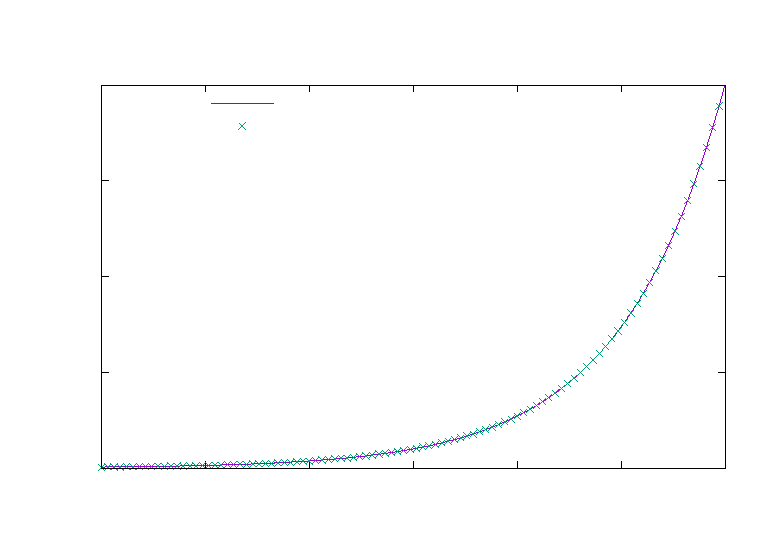
\includegraphics[width={360.00bp},height={252.00bp}]{figures/ex_plot}}%
    \gplfronttext
  \end{picture}%
\endgroup

    \caption{The approximation is very precise}
    \label{fig:result}
\end{figure}


\section{Results}
For moderate values of x the approximation is very precise. The deviation of $ex(x)$ from $exp(x)$ is so small we have no chance of observing the difference in a direct plot of the values as in fig. \ref{fig:result}.



\begin{figure}
   % GNUPLOT: LaTeX picture with Postscript
\begingroup
  \makeatletter
  \providecommand\color[2][]{%
    \GenericError{(gnuplot) \space\space\space\@spaces}{%
      Package color not loaded in conjunction with
      terminal option `colourtext'%
    }{See the gnuplot documentation for explanation.%
    }{Either use 'blacktext' in gnuplot or load the package
      color.sty in LaTeX.}%
    \renewcommand\color[2][]{}%
  }%
  \providecommand\includegraphics[2][]{%
    \GenericError{(gnuplot) \space\space\space\@spaces}{%
      Package graphicx or graphics not loaded%
    }{See the gnuplot documentation for explanation.%
    }{The gnuplot epslatex terminal needs graphicx.sty or graphics.sty.}%
    \renewcommand\includegraphics[2][]{}%
  }%
  \providecommand\rotatebox[2]{#2}%
  \@ifundefined{ifGPcolor}{%
    \newif\ifGPcolor
    \GPcolortrue
  }{}%
  \@ifundefined{ifGPblacktext}{%
    \newif\ifGPblacktext
    \GPblacktextfalse
  }{}%
  % define a \g@addto@macro without @ in the name:
  \let\gplgaddtomacro\g@addto@macro
  % define empty templates for all commands taking text:
  \gdef\gplbacktext{}%
  \gdef\gplfronttext{}%
  \makeatother
  \ifGPblacktext
    % no textcolor at all
    \def\colorrgb#1{}%
    \def\colorgray#1{}%
  \else
    % gray or color?
    \ifGPcolor
      \def\colorrgb#1{\color[rgb]{#1}}%
      \def\colorgray#1{\color[gray]{#1}}%
      \expandafter\def\csname LTw\endcsname{\color{white}}%
      \expandafter\def\csname LTb\endcsname{\color{black}}%
      \expandafter\def\csname LTa\endcsname{\color{black}}%
      \expandafter\def\csname LT0\endcsname{\color[rgb]{1,0,0}}%
      \expandafter\def\csname LT1\endcsname{\color[rgb]{0,1,0}}%
      \expandafter\def\csname LT2\endcsname{\color[rgb]{0,0,1}}%
      \expandafter\def\csname LT3\endcsname{\color[rgb]{1,0,1}}%
      \expandafter\def\csname LT4\endcsname{\color[rgb]{0,1,1}}%
      \expandafter\def\csname LT5\endcsname{\color[rgb]{1,1,0}}%
      \expandafter\def\csname LT6\endcsname{\color[rgb]{0,0,0}}%
      \expandafter\def\csname LT7\endcsname{\color[rgb]{1,0.3,0}}%
      \expandafter\def\csname LT8\endcsname{\color[rgb]{0.5,0.5,0.5}}%
    \else
      % gray
      \def\colorrgb#1{\color{black}}%
      \def\colorgray#1{\color[gray]{#1}}%
      \expandafter\def\csname LTw\endcsname{\color{white}}%
      \expandafter\def\csname LTb\endcsname{\color{black}}%
      \expandafter\def\csname LTa\endcsname{\color{black}}%
      \expandafter\def\csname LT0\endcsname{\color{black}}%
      \expandafter\def\csname LT1\endcsname{\color{black}}%
      \expandafter\def\csname LT2\endcsname{\color{black}}%
      \expandafter\def\csname LT3\endcsname{\color{black}}%
      \expandafter\def\csname LT4\endcsname{\color{black}}%
      \expandafter\def\csname LT5\endcsname{\color{black}}%
      \expandafter\def\csname LT6\endcsname{\color{black}}%
      \expandafter\def\csname LT7\endcsname{\color{black}}%
      \expandafter\def\csname LT8\endcsname{\color{black}}%
    \fi
  \fi
    \setlength{\unitlength}{0.0500bp}%
    \ifx\gptboxheight\undefined%
      \newlength{\gptboxheight}%
      \newlength{\gptboxwidth}%
      \newsavebox{\gptboxtext}%
    \fi%
    \setlength{\fboxrule}{0.5pt}%
    \setlength{\fboxsep}{1pt}%
    \definecolor{tbcol}{rgb}{1,1,1}%
\begin{picture}(7200.00,5040.00)%
    \gplgaddtomacro\gplbacktext{%
      \csname LTb\endcsname%%
      \put(1738,704){\makebox(0,0)[r]{\strut{}$-2.5\times10^{-14}$}}%
      \put(1738,1072){\makebox(0,0)[r]{\strut{}$-2\times10^{-14}$}}%
      \put(1738,1439){\makebox(0,0)[r]{\strut{}$-1.5\times10^{-14}$}}%
      \put(1738,1807){\makebox(0,0)[r]{\strut{}$-1\times10^{-14}$}}%
      \put(1738,2174){\makebox(0,0)[r]{\strut{}$-5\times10^{-15}$}}%
      \put(1738,2542){\makebox(0,0)[r]{\strut{}$0$}}%
      \put(1738,2909){\makebox(0,0)[r]{\strut{}$5\times10^{-15}$}}%
      \put(1738,3277){\makebox(0,0)[r]{\strut{}$1\times10^{-14}$}}%
      \put(1738,3644){\makebox(0,0)[r]{\strut{}$1.5\times10^{-14}$}}%
      \put(1738,4012){\makebox(0,0)[r]{\strut{}$2\times10^{-14}$}}%
      \put(1738,4379){\makebox(0,0)[r]{\strut{}$2.5\times10^{-14}$}}%
      \put(1870,484){\makebox(0,0){\strut{}$-10$}}%
      \put(2363,484){\makebox(0,0){\strut{}$-8$}}%
      \put(2857,484){\makebox(0,0){\strut{}$-6$}}%
      \put(3350,484){\makebox(0,0){\strut{}$-4$}}%
      \put(3843,484){\makebox(0,0){\strut{}$-2$}}%
      \put(4337,484){\makebox(0,0){\strut{}$0$}}%
      \put(4830,484){\makebox(0,0){\strut{}$2$}}%
      \put(5323,484){\makebox(0,0){\strut{}$4$}}%
      \put(5816,484){\makebox(0,0){\strut{}$6$}}%
      \put(6310,484){\makebox(0,0){\strut{}$8$}}%
      \put(6803,484){\makebox(0,0){\strut{}$10$}}%
    }%
    \gplgaddtomacro\gplfronttext{%
      \csname LTb\endcsname%%
      \put(209,2541){\rotatebox{-270}{\makebox(0,0){\strut{}y}}}%
      \put(4336,154){\makebox(0,0){\strut{}x}}%
      \csname LTb\endcsname%%
      \put(3850,4206){\makebox(0,0)[r]{\strut{}$\frac{ex(x)}{exp(x)}-1$}}%
      \csname LTb\endcsname%%
      \put(4336,4709){\makebox(0,0){\strut{}Devation from system math value}}%
    }%
    \gplbacktext
    \put(0,0){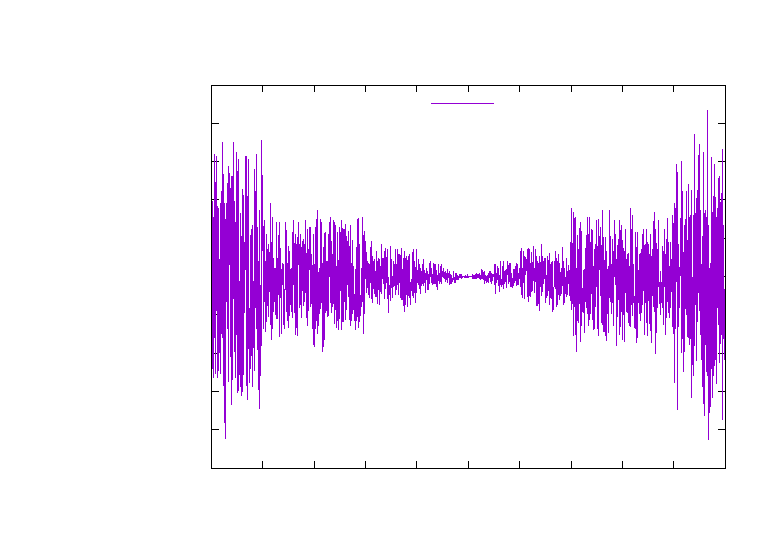
\includegraphics[width={360.00bp},height={252.00bp}]{figures/exerror_plot}}%
    \gplfronttext
  \end{picture}%
\endgroup

    \caption{The relative error rises in steps due to the recursive definition of the approximation}
   \label{fig:result2}
\end{figure}

Instead we consider the relative deviation from the system math value of $exp(x)$, see fig. \ref{fig:result2}. We notice that the deviation is larger for larger absolute values of x. The deviation rises in steps, which is natural since the approximation for each octave interval $]2^{n},2^{n+1}]$ is inherited from the previous down to the 'mould' of the approximation at $]2^{-4},2^{-3}]$. Since
\begin{equation}
    \frac{ex(2x)}{exp(2x)} = \left( \frac{ex(x)}{exp(x)} \right)^2
\end{equation}
we can estimate the deviation at $e^{709} \approx 1 \times 10^{308}$, the largest double allowed in \texttt{C\#}. The approximation for this value is six 'generations' up from the the $]8,16]$-interval which we read from fig. \ref{fig:result2} to have a relative deviation at about $1 + 1.5 \times 10^{-14}$. Hence, using
$(1 + \epsilon)^2 \approx (1 + 2 \epsilon)$ the relative deviation at the maximum calculable value will be about $1 + 9.6 \times 10^{-13}$. Not that bad.




\section{Conclusion}
We have successfully shown that $e^x$ can be estimated using only multiplications and additions. 


\end{document}